\chapter{Обзор существующих решений рассматриваемой задачи или её модификаций}
\label{cha:ch_2}
%Эта работа во многом является повторением исследования из статьи о детекции эффекта 
%Сюняева-Зельдовича \cite{Bonjean}, с той разницей, что здесь будут использоваться оптические данные, в то время 
%как в упомянутой статье использовались данные микроволнового диапазона.\\

В первую очередь рассмотрим работу о детекции эффекта Сюняева-Зельдовича \cite{Bonjean}. Её автор 
тоже использует для сегментации данных архитектуру U-net. \\

Основной целью описываемой работы являлось создание алгоритма для детекции источников через эффект 
Сюняева-Зельдовича по данным телескопа <<Планк>>. Соответственно, кроме самих обзоров неба, полученных 
<<Планком>>, использовались еще три каталога скоплений для создания целевых данных:

\begin{enumerate}
	\item PSZ2. Этот каталог был получен по данным <<Планка>>  при помощи алгоритмов 
	согласованного мультифильтра и PowellSnakes.
	\item MCXC (Meta-Catalogue of X-ray detected Clusters). Это объединенный каталог из всех 
	других каталогов скоплений, полученных из данных телескопа ROSAT.
	\item RedMaPPer (Red-sequence Matched-filter Probabilistic Percolation). Каталог скоплений, 
	полученный с помощью одноимённого алгоритма из данных оптического диапазона.
\end{enumerate}

Несмотря на то, что в этих каталогах содержатся данные об объектах, детектированных в разных 
диапазонах, они содержат довольно большое количество общих объектов (поэтому при создании 
тренировочных выборок нужно удалять из каталогов повторы). \\

В описываемой работе для создания тренировочных выборок использовалось разбиение неба проекцией 
HEALPix (Hierarchical Equal Area isoLatitude Pixelisation). \\
\begin{figure}[h]
	\center{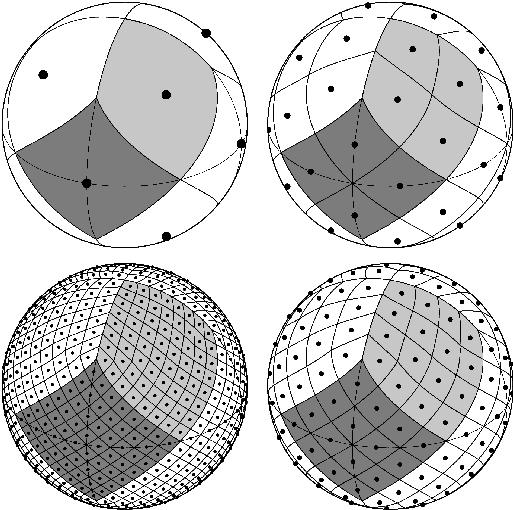
\includegraphics[width=5cm]{healpix0}}
	\caption{Примеры разбиения сферы HEALPix \cite{Healpix}}
\end{figure}

Разбиение с параметром $n_{side}=2$ позволяет получить 48 больших областей неба. Некоторые из них 
были использованы для тестирования полученной модели и для валидации, все остальные были 
использованы для обучения модели.\\ 

Случайным образом в соответствуюхих областях разбиения HEALPix выбирались центры патчей и их 
ориентации для создания тренировочных, валидационных и тестовых выборок. Каждый патч представлял 
из себя изображение размера 64 x 64 с шестью каналами различных данных. Размер каждого пикселя 
на таких патчах составлял 1.7 arcmin. \\

После этого 100000 патчей были использованы для обучения нейросети. Обучение длилось более 30 эпох. \\ 
\begin{figure}[h!]
	\center{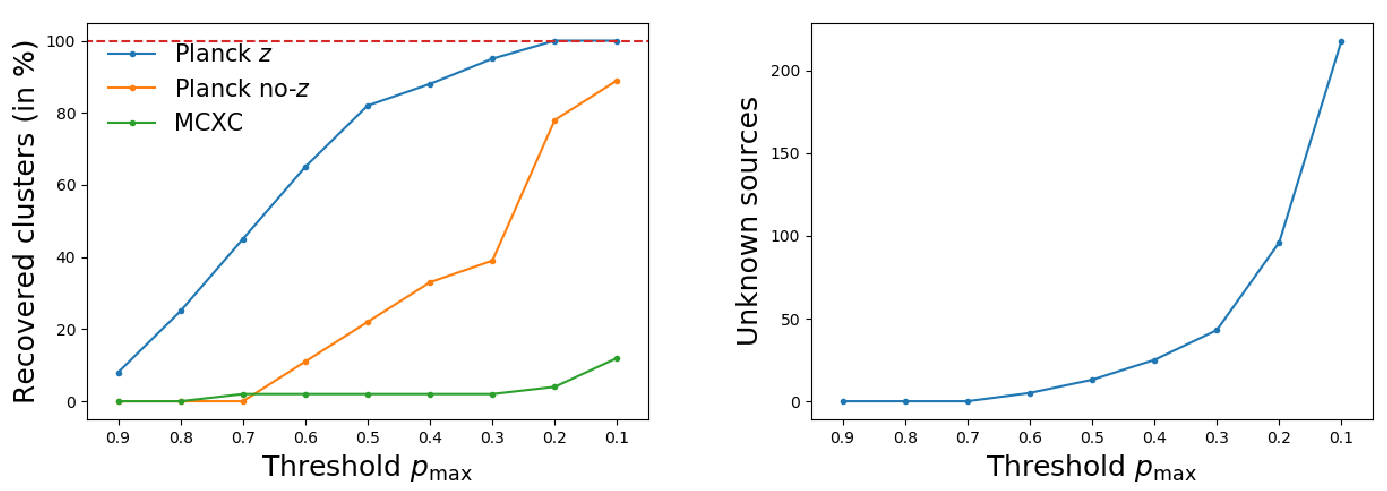
\includegraphics[width=15cm]{sz0}}
	\caption{Результаты исследования работы \cite{Bonjean}}
\end{figure}

Как можно увидеть из результатов, лучше всего нейросеть сегментирует в данных телескопа <<Планк>> 
скопления из каталога того же самого <<Планка>>.\\

В описываемой статье использовалась классическая версия архитектуры U-net: каждый из блоков 
кодировщика состоит из двух свёрток с ядром 3 x 3 с последующими активациями ReLU после каждой 
свёртки за ними следует слой MaxPooling для уменьшения размерности входных данных. Всего в 
кодировщике пять таких блоков. Блоки декодировщика состоят из слоя Upsampling, повышающего 
размерность предыдущего слоя, конкатенации выхода из кодировщика с соответсвующими размерами и 
так же двух сверток с ReLU. Кроме того, после каждого слоя свёртки добавлен слой Dropout с 
параметром 0.2 для предотвращения переобучения. После всех блоков декодировщика добавляется слой 
активации сигмоиды для последующего использования кросс-энтропии как loss-функции. Количество 
фильтров для первого блока варьировалось от 8 до 128.\\

Для детекции скоплений на полученных из нейросети данныx, зонами скоплений обозначались зоны, 
занимающие пиксели со значением больше $p_{max}$, а затем на них находились барицентры, которые 
впоследствии считались предсказанными центрами скоплений. Таким образом большая часть скоплений из 
каталога PSZ2 была успешно распознана нейросетью. \\
